\setchapterpreamble[u]{\margintoc}
\chapter[System Stability ($4^{th}$ Lecture)]{System Stability}
\labch{lec4}

\section{Singularities of a Function}
\labsec{sec4.1}

System is stable if for bounded input the output is bounded BIBO.
System stability can be determined from the Transfer Function.\\[+1em]

$T.F = \dfrac{N(s)}{D(s)} = \dfrac{b_ms^m+b_{m-1}s^{m-1}+\ldots+b_1s+b_o}{a_ns^{n\ }+a_{n-1}s^{\ n-1}+\ldots+a_1s+a_o}$\\[+1em]

Can be written in terms of factors:\\[+1em]

$T.F = \dfrac{N(s)}{D(s)} = K \dfrac{(s-Z_1)(s-Z_2)\ldots(s-Z_{m-1})(s-Z_m)}{(s-P_1)(s-P_{2\ }\ldots(s-P_{\ n-1})(s-P_{n\ })}$\\[+1em]

-> Roots of $D(s): P_1, P_2, \ldots, P_n$ are called poles.\\
-> Roots of $N(s): Z_1, Z_2, \ldots, Z_m$ are called zeros.\\
\note{where $m<n$}\\

All coeffieceints of $D(s), N(s)$ are real -> poles and zeros must be real or complex conjugate.\\[+1em]

$T.F = K ( \dfrac{A_1}{S-P_1} + \dfrac{A_2}{S-P_2} + \ldots + \dfrac{A_{n-1}}{S-P_{n-1}} + \dfrac{A_n}{S-P_n} )$\\[+1em]

For a second order systems: Root $ ( - \omega_n [\zeta \pm \sqrt{\zeta^2-1}] ) $ 

\begin{figure*}[!h]
	\raggedleft
	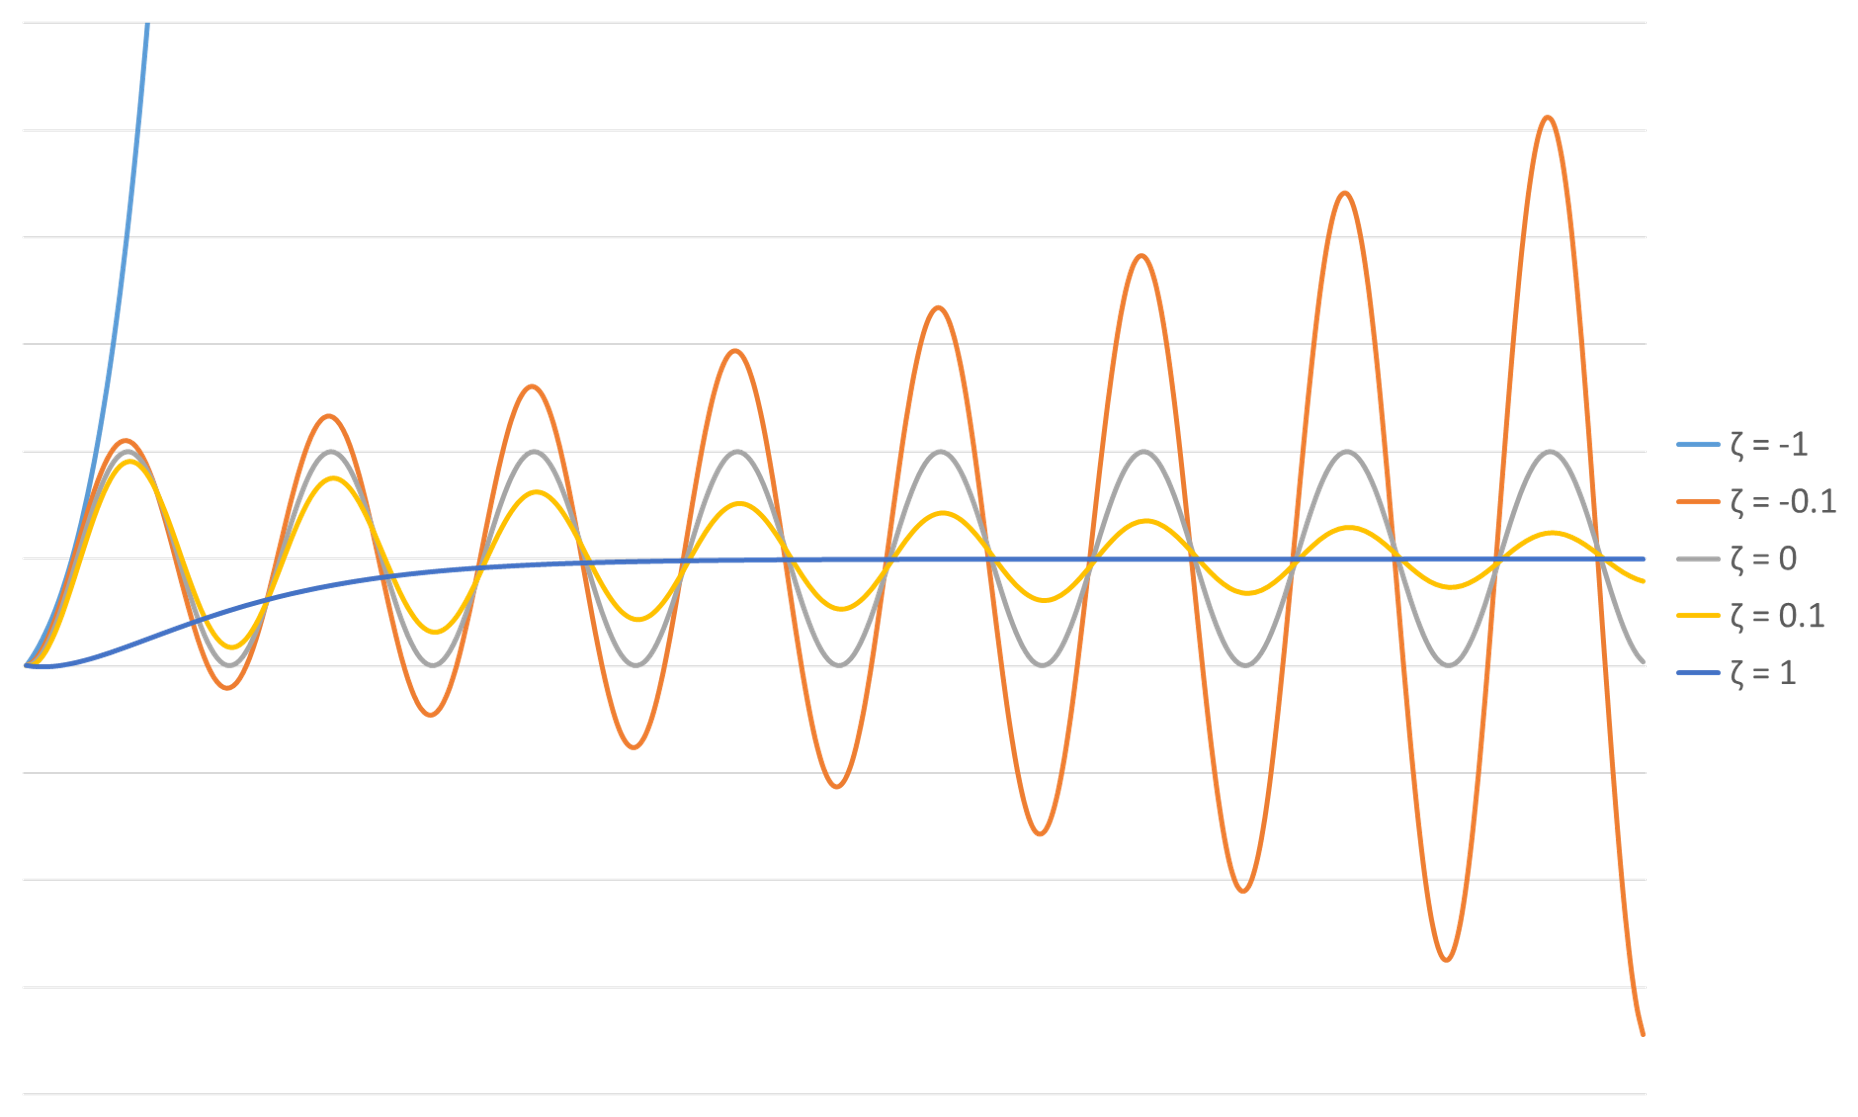
\includegraphics[width=8cm]{lec4/Picture1}
\end{figure*}

$F(s)=\dfrac{A}{s}$

Root is zero ($ s = 0 $):\\

-> unstable: $\displaystyle{\int_0^\infty f(t)\ dt\ }$ is not bounded.\\[+1em]

Stability Condition:\\

all poles lie in the left half of s-plane\\

-> all coefficients of $D(s)$ must be real and positive.\\

-> all powers of s from $s^1$ to $s^n$ should be present, however all odd powers of s or all even power of s may be missing.\\
\note{necessary conditions, but not sufficient}

\section{Routh's Stability Criterion}
\labsec{sec4.2}

\subsubsection{Ref}

The higher the degree of $D(s)$, the more laborious is the process of finding its factors.\\

The stability of the response requires that all roots of $D(s)$ have negative real parts.\\

If such roots of $D(s)$ with positive real parts are found, the system must be modified. Routh's
criterion is a simple method of determining the number of roots with positive real parts without
actually solving for the roots of $D(s)$.\\

\subsubsection{Slides}

The Routh-Hurwitz criterion states that 
``the number of roots of the characteristic equation with positive real parts is equal to the
 number of changes in sign of the first column of the Routh array''.

\begin{table*}[!b]
	\begin{tabular}{p{16cm}}
		\multicolumn{1}{m{16cm}}{\LARGE{$This\ is\ the\ last\ lecture,\ I\ will\ personally\ depend\ on$}}\\[+1em]
		\multicolumn{1}{r}{
			\fbox{
			    \parbox{8.2cm}{
			    	\LARGE{\href{https://drive.google.com/drive/folders/1G3lhSEKO3itcgrWF_8Sl6ArfrC4g3E8-}{$\ Dr.\ Imtiaz\ Hussain\ Lectures\ $}}
		    	}
			}
		}
		
	\end{tabular}
\end{table*}
